\begin{frame}{Modello matematico}
	\begin{block}{Dinamica di portafoglio}<1-2>
		\begin{equation*}
		x_{k+1} = x_k(1+\bm{u}_k^T\bm{w}_{k+1}), \quad k \in \mathbb{N}
		\end{equation*}
	\end{block}
	dove
	\begin{itemize}
		\item $x_k$ stato del sistema e valore del portafoglio al'istante $k\in \mathbb{N}$
		\item $\bm{u}_k$ variabile di controllo del sistema e vettore dei pesi di portafoglio
		\item $\bm{w}_{k+1}$ vettore dei rendimenti dei titoli
	\end{itemize}
	\begin{block}{Obiettivo}<2>
		\begin{equation*}
		\Optmax_{\pi \in \mathcal{U}_{N-1}} \mathbb{P}\Big(\big\{\omega \in \Omega : x_0 \in X_0,\ldots,x_N \in X_N \big\} \Big).
		\end{equation*}
	\end{block}
\end{frame}	


\begin{frame}{Modello Matematico}
	\begin{block}{Optimal Dynamic Asset Allocation (ODAA) Algorithm}
		\begin{align*}
		J_N(x) & = \mathbbm{1}_{X_N}(x) \nonumber \\
		J_k(x) & = \sup_{\bm{u}_k \in U_k}\int_{X_{k+1}}J_{k+1}(z)p_{f(x,\bm{u}_k,\bm{w}_{k+1})}(z)\mathrm{d}z \\
		& \forall k = N-1,\ldots,1,0. 
		\end{align*}
	\end{block}
    \begin{columns}
	    \begin{column}{.5\textwidth}
	    	In output l'algoritmo fornisce la \textbf{strategia ottima} 
	    	\[ \pi^{\star} =  \{\mu_0^{\star},\ldots,\mu_{N-1}^{\star} \},  \]
	    	ossia una sequenza di mappe \[  \mu_k^{\star} \colon x \mapsto \bm{u}_{k}^{\star}, \quad \forall k  \]
	    \end{column}
	    \begin{column}{.5\textwidth}<2>
	    	\begin{alertblock}{Elevato costo computazionale}
	    		un'ottimizzazione vincolata $\forall k = 1,\ldots,N-1, \quad \forall x \in X_k$
	    	\end{alertblock}
	    \end{column}
    \end{columns}
	
\end{frame}

\begin{frame}{Modello di mercato}
	I rendimenti delle asset class $\bm{w}_{k+1}$ vengono modellizzati con una \textbf{Mistura Gaussiana}:
	\begin{block}{}
		\begin{equation*}
		p_{\bm{w}_{k+1}} = \lambda\varphi_{(\bm{\mu_1},\bm{\Sigma}_1)} + (1-\lambda)\varphi_{(\bm{\mu_2},\bm{\Sigma}_2)}, \quad \lambda \in [0,1]
		\end{equation*}
	\end{block}
	\begin{figure}
		\centering
		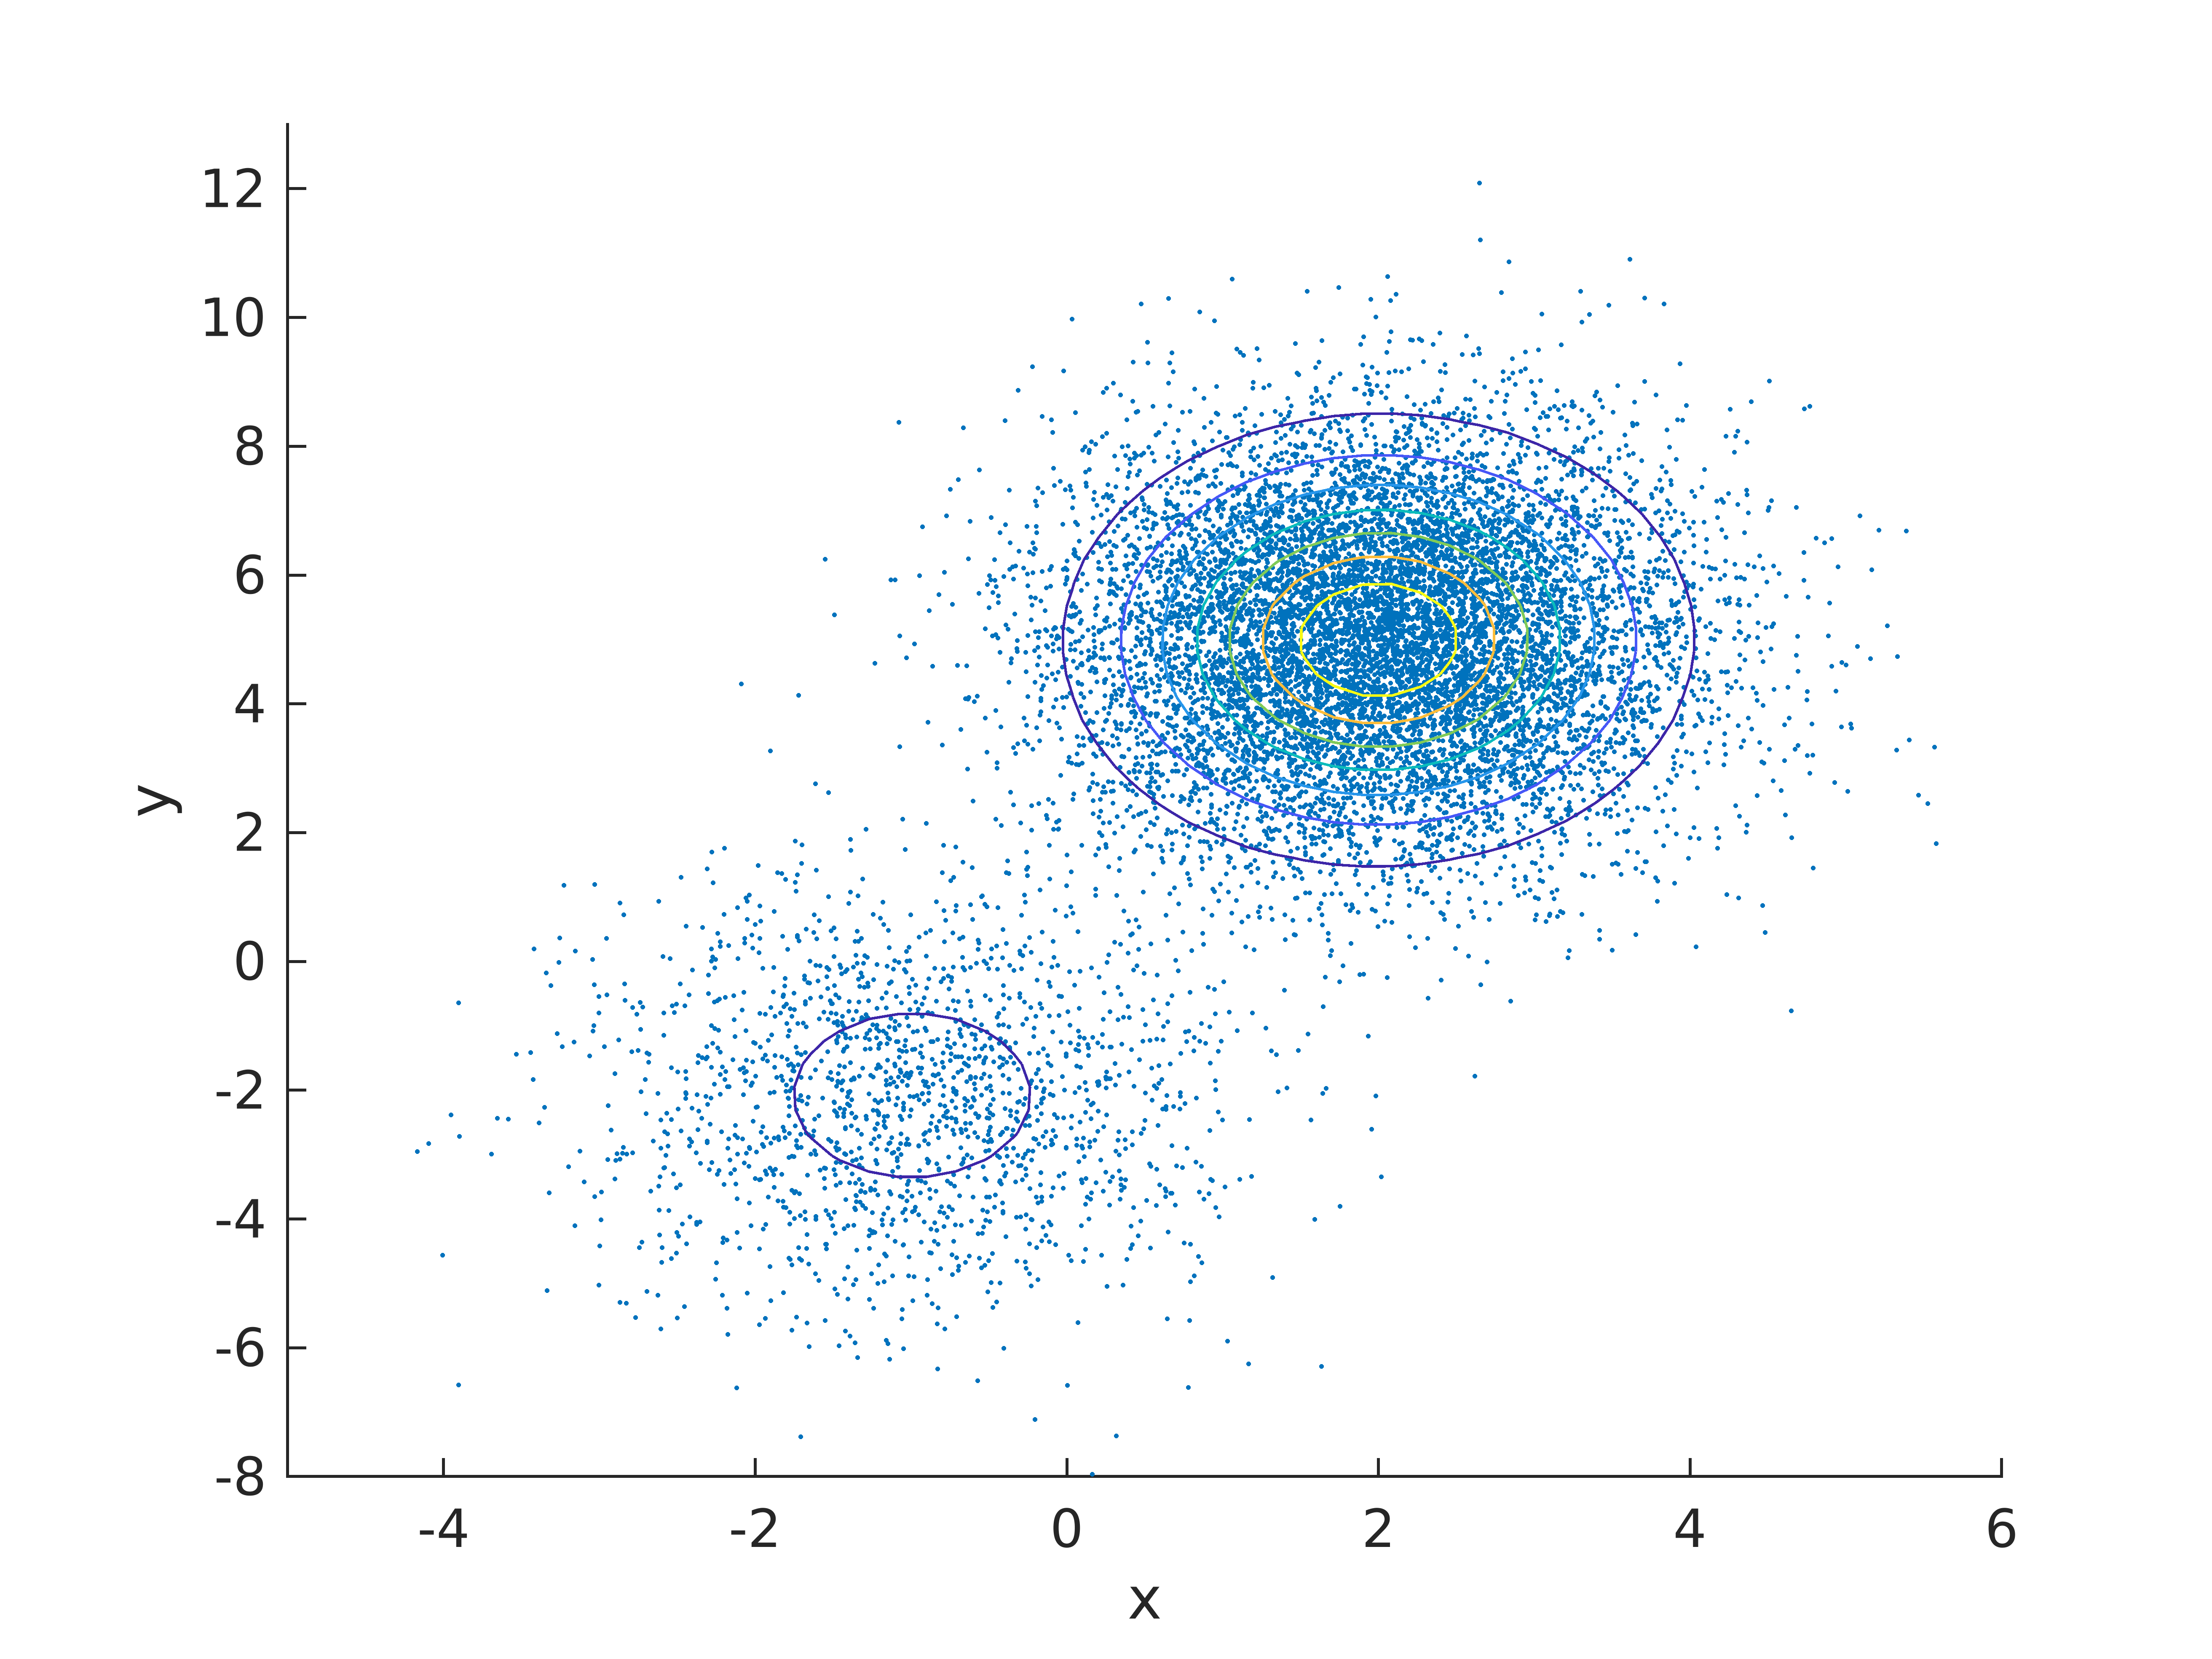
\includegraphics[width=0.65\linewidth]{Images/Scatter}
	\end{figure}
	
	
\end{frame}	

\begin{frame}{Mappe di Allocazione: }
	\begin{columns}
		\begin{column}{0.35\textwidth}
			\textbf{parametri investimento}:
				\begin{itemize}
					\item orizzonte 2 anni
					\item ribilanciamento settimanale
					\item  $x_0=1$
					\item target return 7\% annuo
					\item $V@R_{1-\alpha} = 7\%$
				\end{itemize}
			
			\textbf{probabilità raggiungimento target}:
			$p^{\star} = 78.59\%$
			
		\end{column}
		\begin{column}{0.65\textwidth}
			\begin{figure}
				\centering
				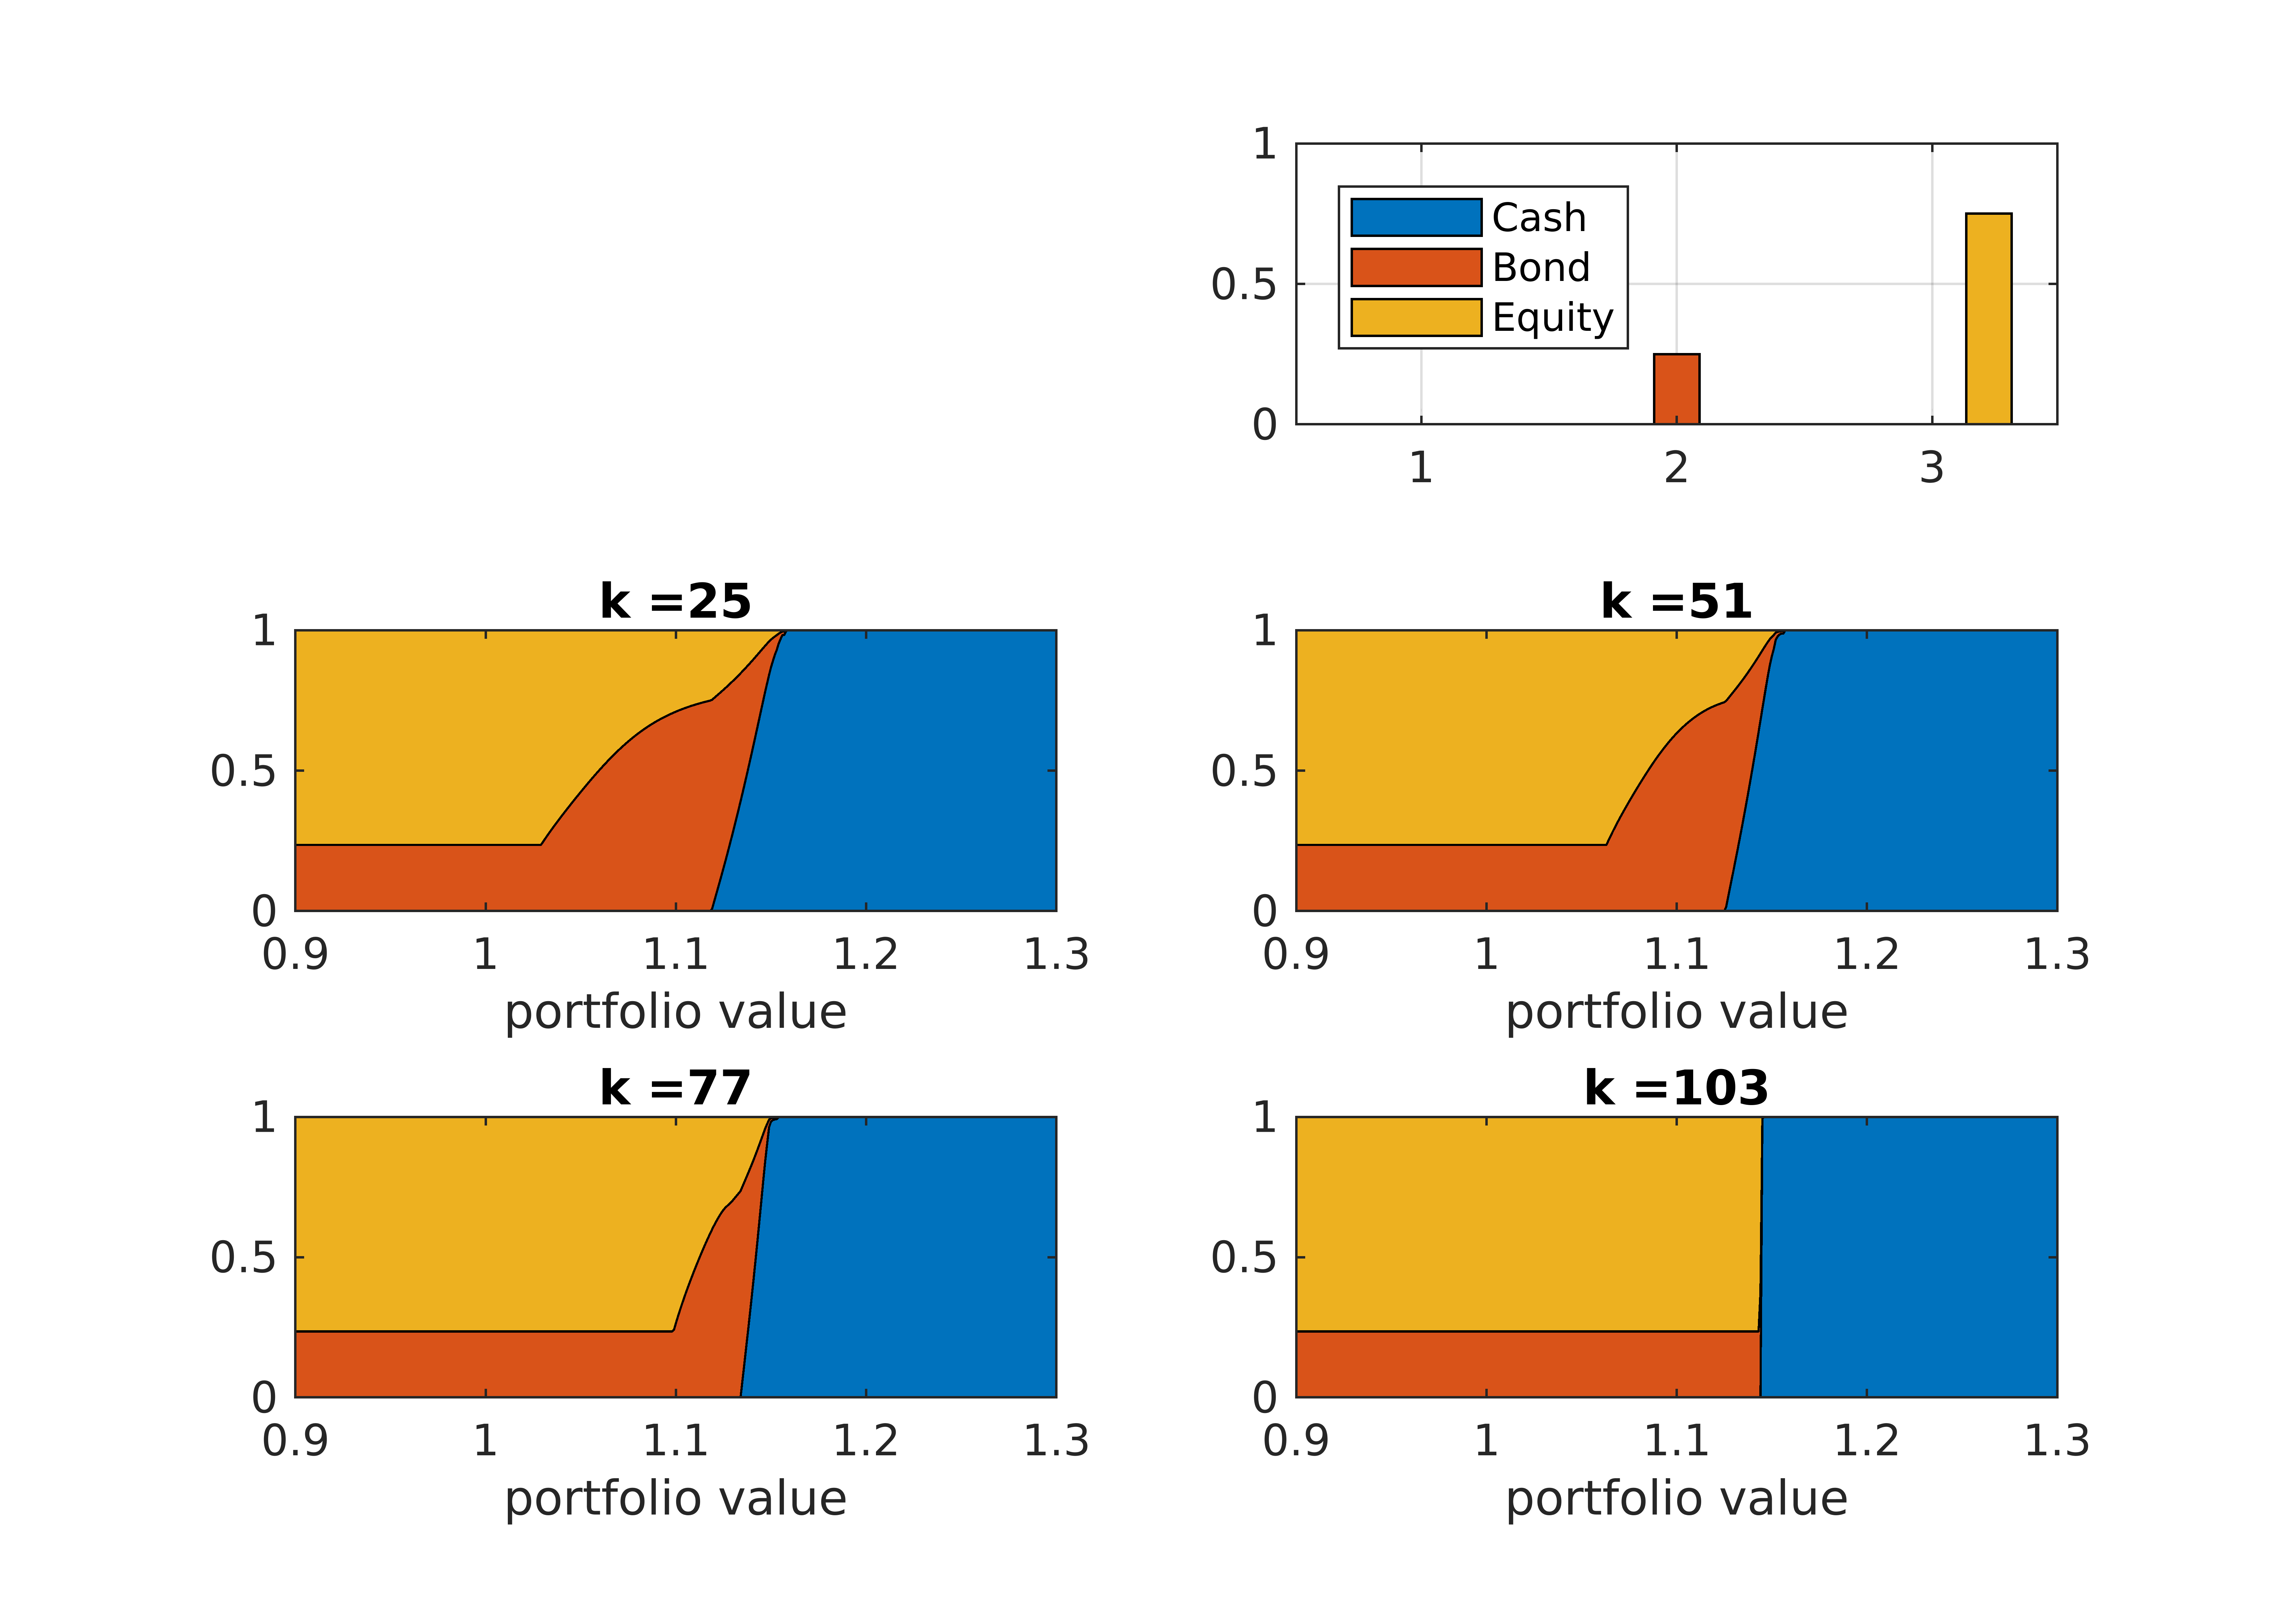
\includegraphics[height=5.5cm]{Images/mapsMixturewk}
			\end{figure}
		\end{column}
	\end{columns}
	
	
\end{frame}

\begin{frame}{Simulazione Monte Carlo}
	\begin{figure}
		\centering
		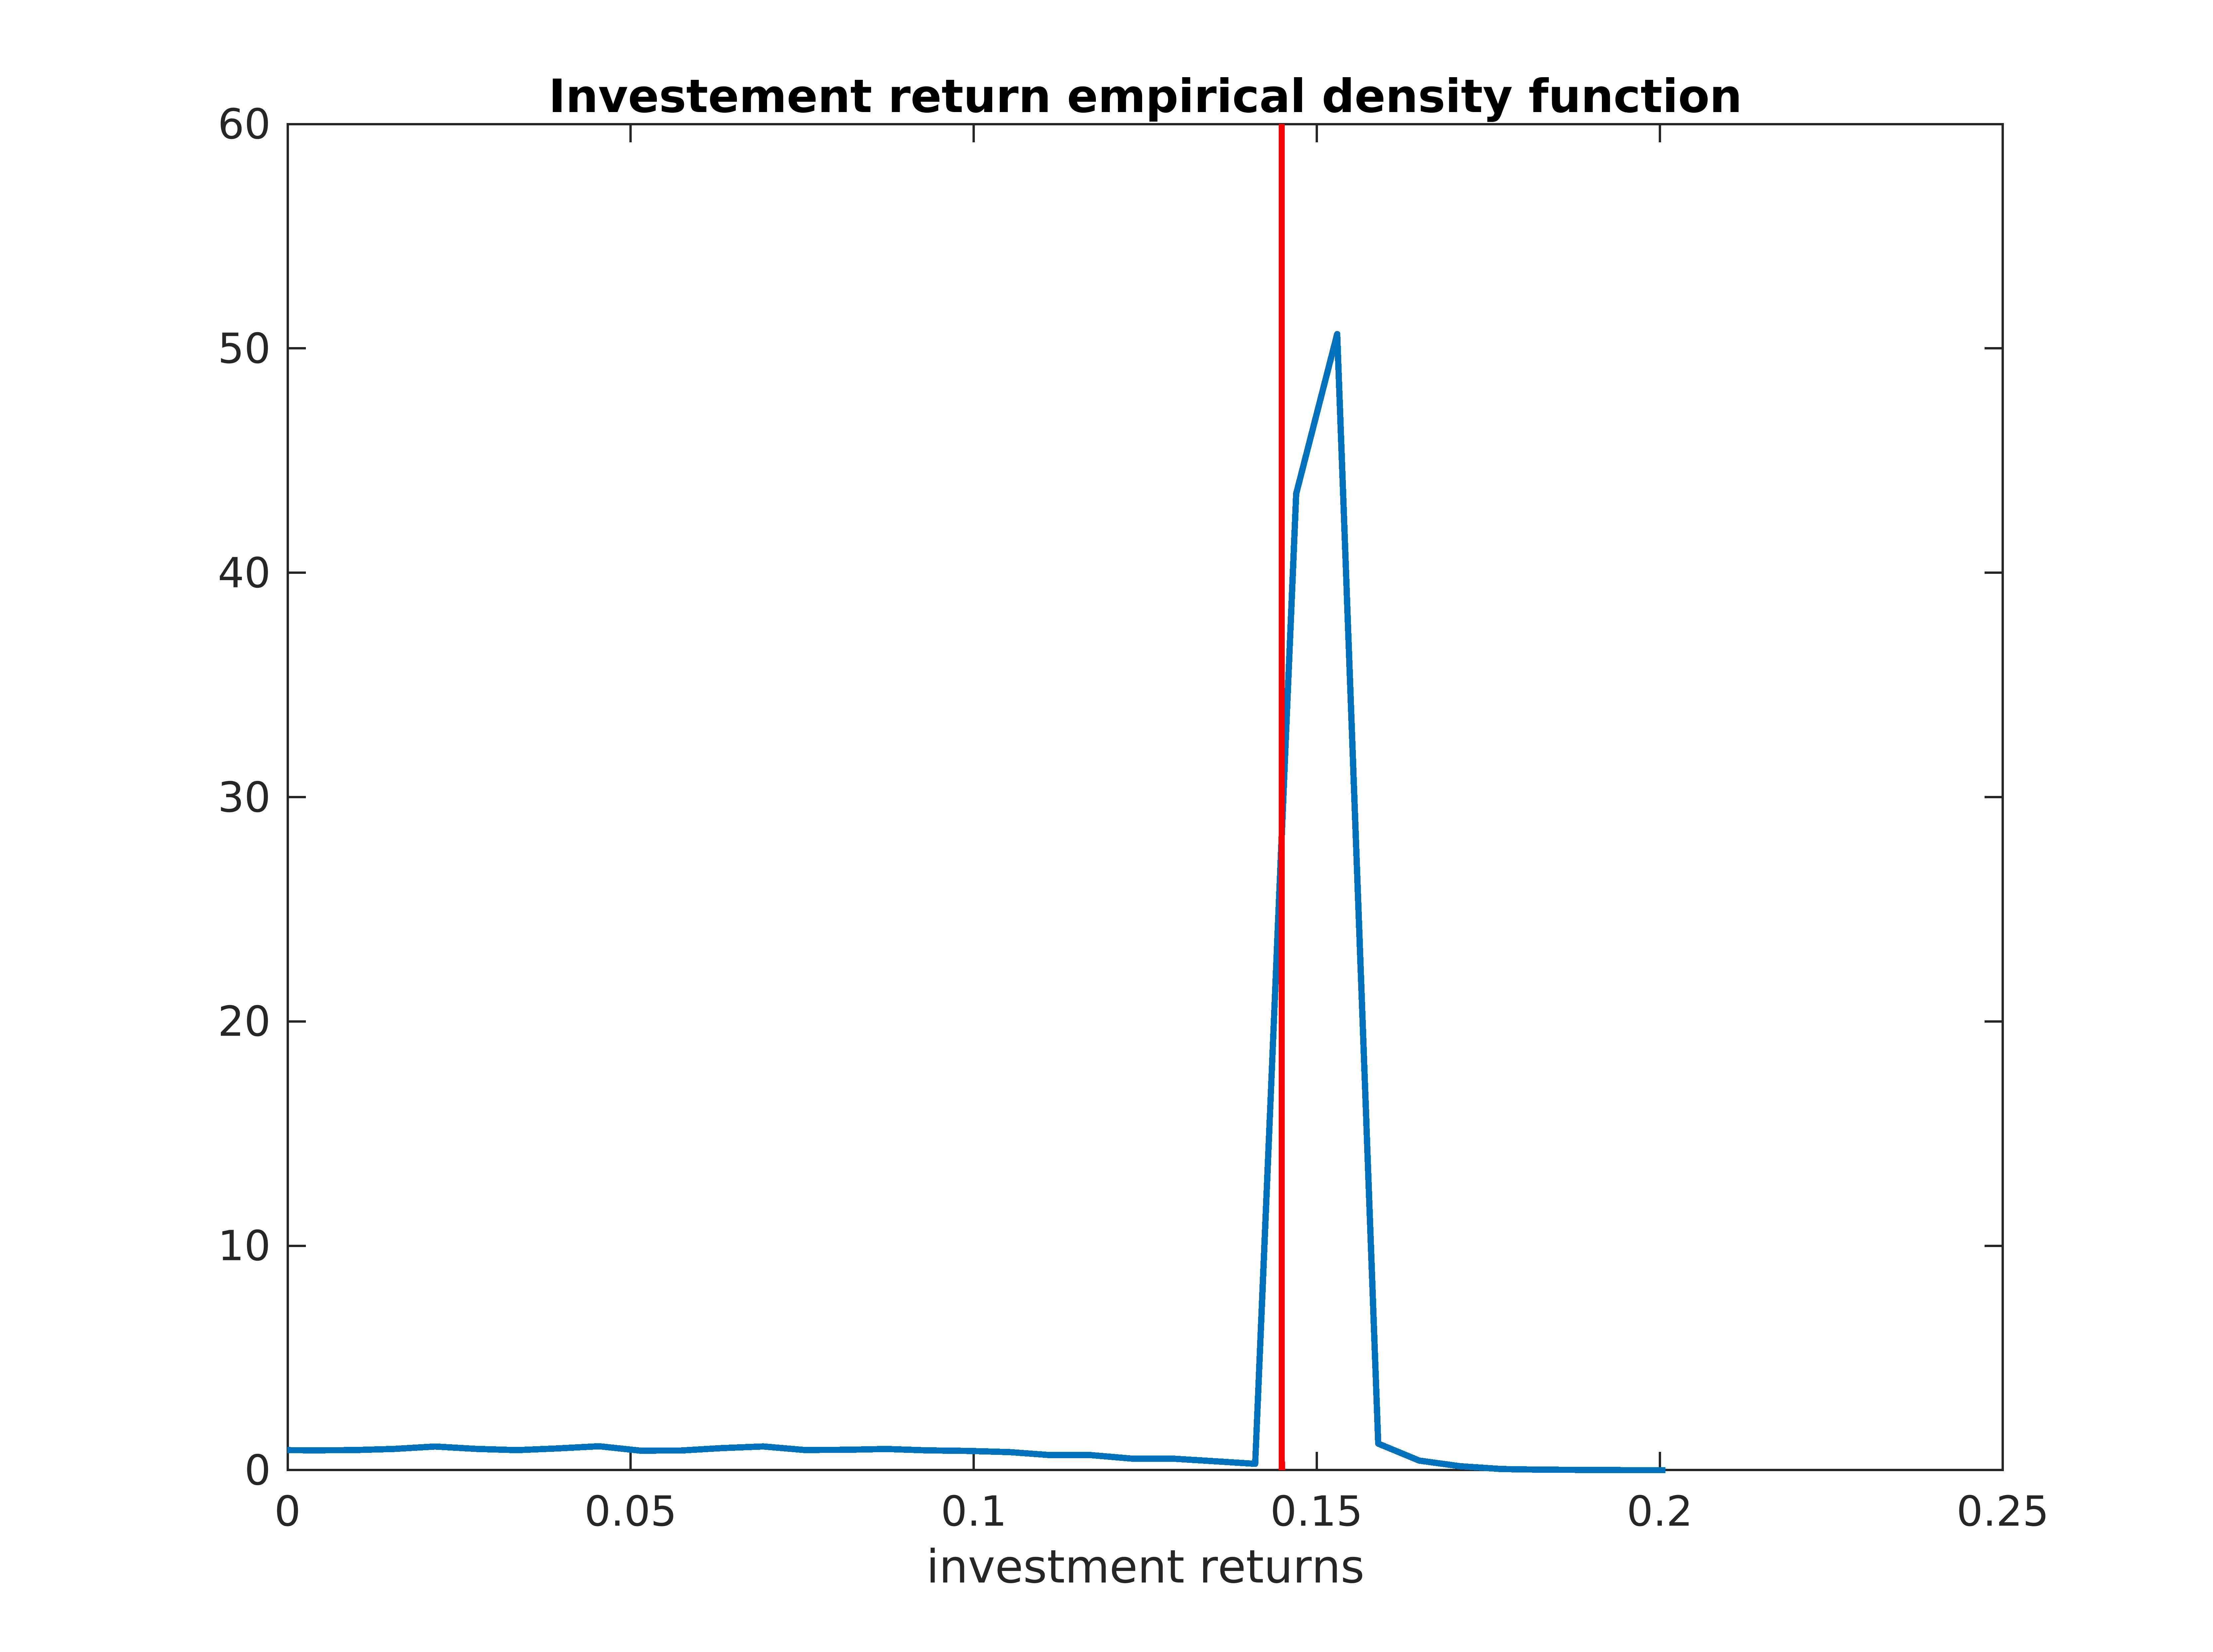
\includegraphics[width=0.8\linewidth]{Images/DensityODAAwk}
	\end{figure}
\end{frame}

	